%%%%%%%%%%%%%%%%%%%%%%%%%%%%%%%%%%%%%%%%%
% CN2 Labreport template
%
% License:
% CC BY-NC-SA 3.0 (http://creativecommons.org/licenses/by-nc-sa/3.0/)
%
%%%%%%%%%%%%%%%%%%%%%%%%%%%%%%%%%%%%%%%%%

\documentclass[parskip=full]{scrartcl}

\usepackage{siunitx}  % Provides the \SI{}{} command for typesetting SI units
\usepackage{graphicx} % Required for the inclusion of images
\usepackage{booktabs} % nicer tables
\usepackage[noabbrev]{cleveref} % automatic references
\usepackage{listings} % typeset code
\usepackage[backend=biber]{biblatex}
\addbibresource{referenzen.bib}

\crefname{lstlisting}{listing}{listings} % for referencing code
\Crefname{lstlisting}{Listing}{Listings} % for referencing code

\usepackage[headsepline]{scrlayer-scrpage} % header
\ohead{Group 06} % right part of header
\ihead{Assignment 2} % left part of header

\lstset{basicstyle=\ttfamily} % monospaced font in listing



%----------------------------------------------------------------------------------------
%	DOCUMENT INFORMATION
%----------------------------------------------------------------------------------------

\begin{document}
\begin{titlepage}
    \centering
    \vspace*{2cm}
    {\Huge \textbf{Communication Networks 2}}\\
    SS 2021\\
    \vspace*{1cm}
    {\Large Assignment 2}
    \\\vspace*{3cm}
    {\Large \textbf{Group 06}}\\
    \vspace*{1cm}
    {\large 
        \begin{tabular}{l c c}
            Name & Mat.Nummer \\ \hline
            Paul Kloker & 12034928 \\
            Juan Aramis Oposich & 11701238
        \end{tabular}
    }
    \\\vspace*{7cm}
    \today
\end{titlepage}

%----------------------------------------------------------------------------------------
%	SECTION 1
%----------------------------------------------------------------------------------------
\section{Task description} \label{sec:task}
The task of this assignment is to set up a Voice over IP (VoIP) Client and compare the influence of multimedia codecs on the Quality of Service (QoS) of video calls.
Furthermore, the signaling messages of the Session Initiation Protocol (SIP) shall be analyzed to verify the correct behavior and to find a secret message of the registrar.

The comparison of the QoS is to be done once subjectively and once on the basis of self-selected network parameters, which are also to be visualized graphically. 


%----------------------------------------------------------------------------------------
%	SECTION 2
%----------------------------------------------------------------------------------------
\section{Procedure} \label{sec:procedure}

\subsection{Linphone setup and SIP registration} \label{subsec:setup}
Before a VoIP call can be done, one of the first thing is to do a SIP registration. SIP Endpoints are identified by their Address of Record, for example "sip:cn\_06@cn2lab.cn.tuwien.at".

The endpoint is also defined by the location, which is identified by an IP address, port number and protocol. To receive calls, the caller needs to know the location of the callee. Since most SIP endpoints do not have a permanent, fixed, publicly-reachable IP address, they will need to register with a central server, or Registrar, so that they can receive incoming calls. This server accepts REGISTER requests and places the information it receives in those requests into the location service for the domain it handles. In figure \labelcref{fig:SIP Registrar} the SIP registration flow can be seen. 

\begin{figure}[!ht]
	\centering % centering figure 
	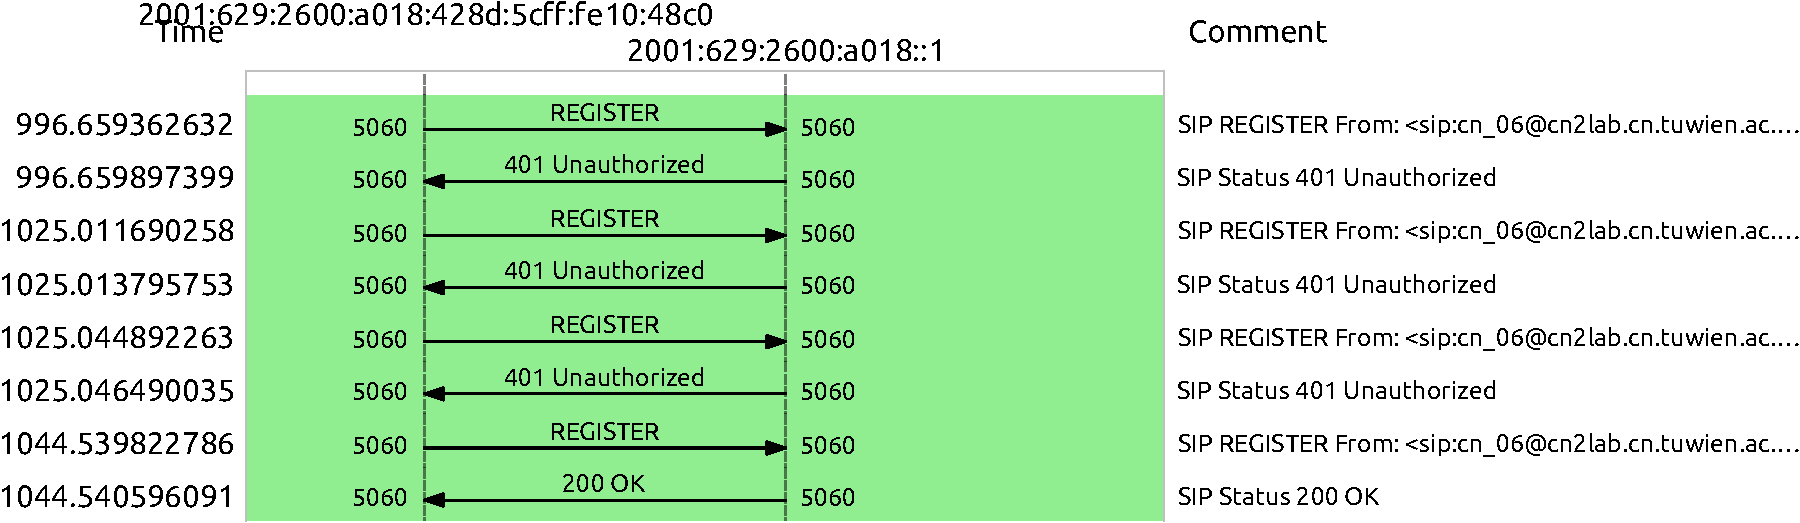
\includegraphics[width=\textwidth]{images/FlowSeqReg.pdf} % importing figure
	\caption{SIP registration flow} 
	\label{fig:SIP Registrar} % labeling to refer it inside the text
\end{figure}

The first sequence is the initial registration request from SIP User Agent with it's address information, the first SIP registrar answers with the information about the login "401 Unauthorized". To be authenticate, the client will combine the received nonce with his user and password information and create an MD5 hash out of them. As the figure above indicates, there has been two failed login for the registration. The last "200 OK" response state a successful login.

\subsubsection{secret message}
One of the task was to extract a secret message from the registration process. This message has been embedded in the last "200 OK" response of the SIP registrar. An additonal header filed, called Message header contained the cleartext information.

\begin{itemize}
	\item Session Initialisation Protocol(20) $\to$ Message Header $\to$ Secret-Message: Dazecixaru4
\end{itemize}

\subsection{Capturing process} \label{subsec:capture}
This year because of the COVID-19 pandemic it was only possible to access the lab PCs remotely.
This is most of the time no problem but to compare the video and audio quality of SIP calls it is important to have direct access, because the VNC connection influences the subjective impressions.
To overcome this problem a command line tool called \verb|cn2_sbs_capture| has been provided, which captures the incoming audio and video and the outgoing video.
Because the camera and microphone of the lab PC could not be used the same video was played each call.

To capture a call, the selected codecs were first set in the Linphone settings. 
Then \verb|cn2_sbs_capture| was executed with the default settings and the Wireshark capture was started. 
After that a one-minute-long call was made. 
Table \ref{tab:capture} shows all captured calls and the chosen codecs.

\begin{table}[hb]
	\centering
	\begin{tabular}{|l|l|l|l|l|l|p{0.25\textwidth}|}
		\hline
		\textbf{No.} & \textbf{type} & \textbf{v. codec} &\textbf{v. score} & \textbf{a. codec} & \textbf{a. score} & \textbf{comment} \\ 
		\hline
		1 & landline & VP8 &5& OPUS &4&- \\
		\hline
		2 & satellite & VP8 &1 &  OPUS &3&no fluent video just single frames every view seconds\\
		\hline
		3 & landline & MP4V\_ES &5& speex 16 kHz &3&-\\
		\hline
		4 & satellite & MP4V\_ES &2& speex 16 kHz &2& fluent video but with many large artifacts \\
		\hline
		5 & landline & MP4V\_ES &5& PCMU &2& -\\
		\hline
		6 & satellite & MP4V\_ES &2& PCMU &1& audio stream sometimes stops\\
		\hline
		7 & satellite & H.263-1998 &2& GSM&1& fluent video but reduced resolution\\
		\hline
		8 & satellite & H.263 &1& speex 8 kHz&2& no video at all\\
		\hline
	\end{tabular}
	\caption{Captured calls (audio $\rightarrow$ a., video $\rightarrow$ v.)}
	\label{tab:capture}
\end{table}

Because capturing all combinations of audio and video codecs would take too much time a selection of codecs was tested independent of each other.
That means we assume the chosen codecs does not influence one another.
This should not be done for precise performance testing.

\subsection{SIP signaling and SDP} \label{subsec:signaling}

To verify that both, signaling and media works correctly and the predefined codecs are used for media transfer, a sequence diagram was created and analyzed for each capture.
Figure \ref{fig:sigFlow} shows the sequence diagram of the SIP signaling and the media flows during the call with the VP8 video codec and the OPUS audio codec over landline. 
It was created by using the Wireshark SIP Flows tool. 
A deeper look in the SDP section in the body of the third message in the flow confirms that the offered codecs in the \verb|INVITE| message were accepted by the callee.

\begin{figure}[!ht]
	\centering % centering figure 
	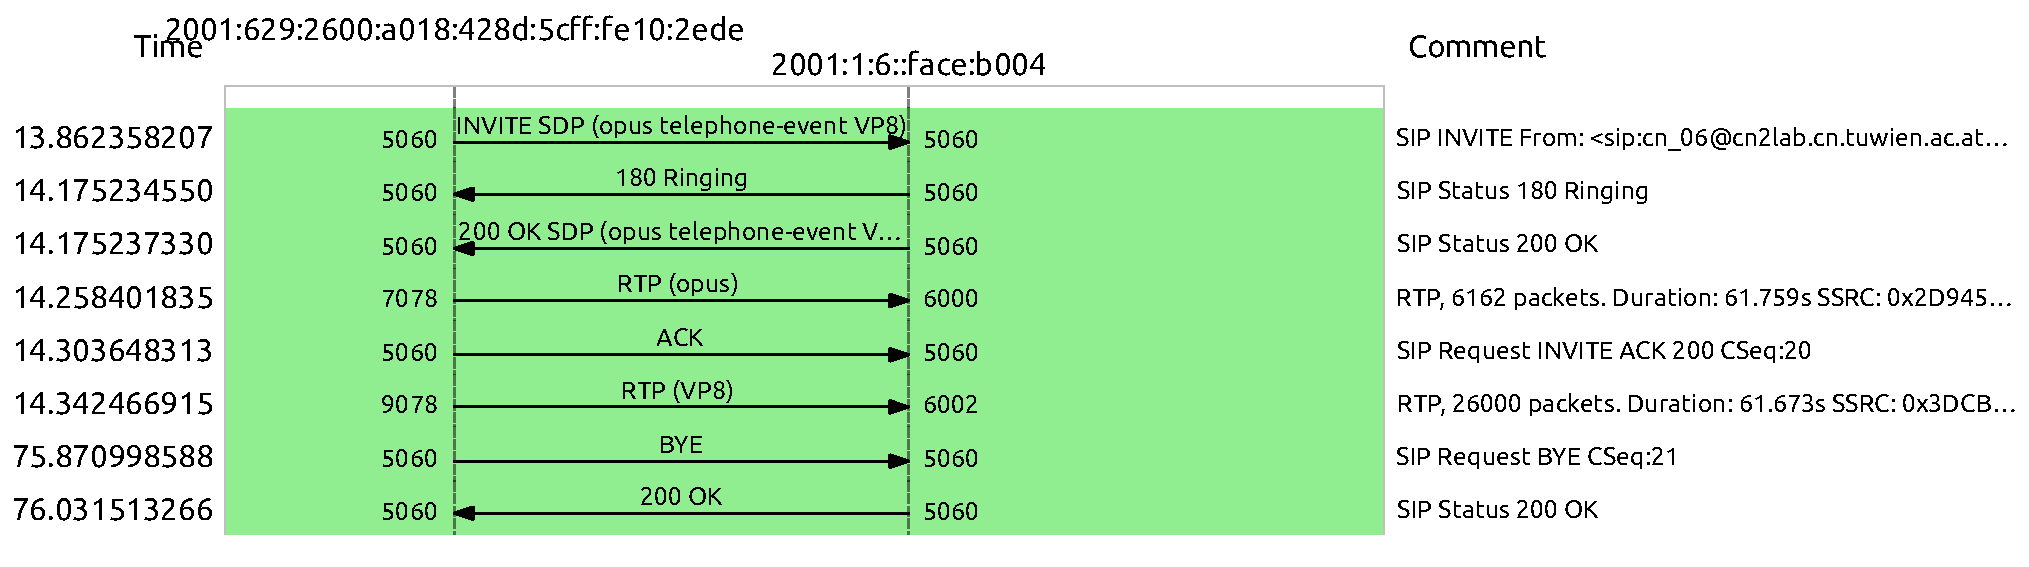
\includegraphics[width=\textwidth]{images/VP8_OPUS_landline_flow.pdf} % importing figure
	\caption{SIP signaling sequence diagram} 
	\label{fig:sigFlow} % labeling to refer it inside the text
\end{figure} 
In some calls, especially in the satellite calls, retransmissions of signaling messages could be identified in the auto generated sequence diagram. 
A unexpected behavior which can be seen in \cref{fig:sigFlow} is the order of the \verb|ACK| message and the initial OPUS RTP stream message. 
Actually, the \verb|ACK| is sent directly after a \verb|200 OK| of the offer and answer process but here the OPUS RTP stream starts before the acknowledgment.
This behavior could be seen in most of the other captures as well, but it has no influence on the functionality because the callee already accepted the offered codecs and the \verb|ACK| message is an own transaction and is not bound to the previous messages.

\subsection{QOS Capturing} \label{subsec:QOS}
Tu nur mal die Bilder einfügen

\begin{figure}[!ht]
	\centering % centering figure 
	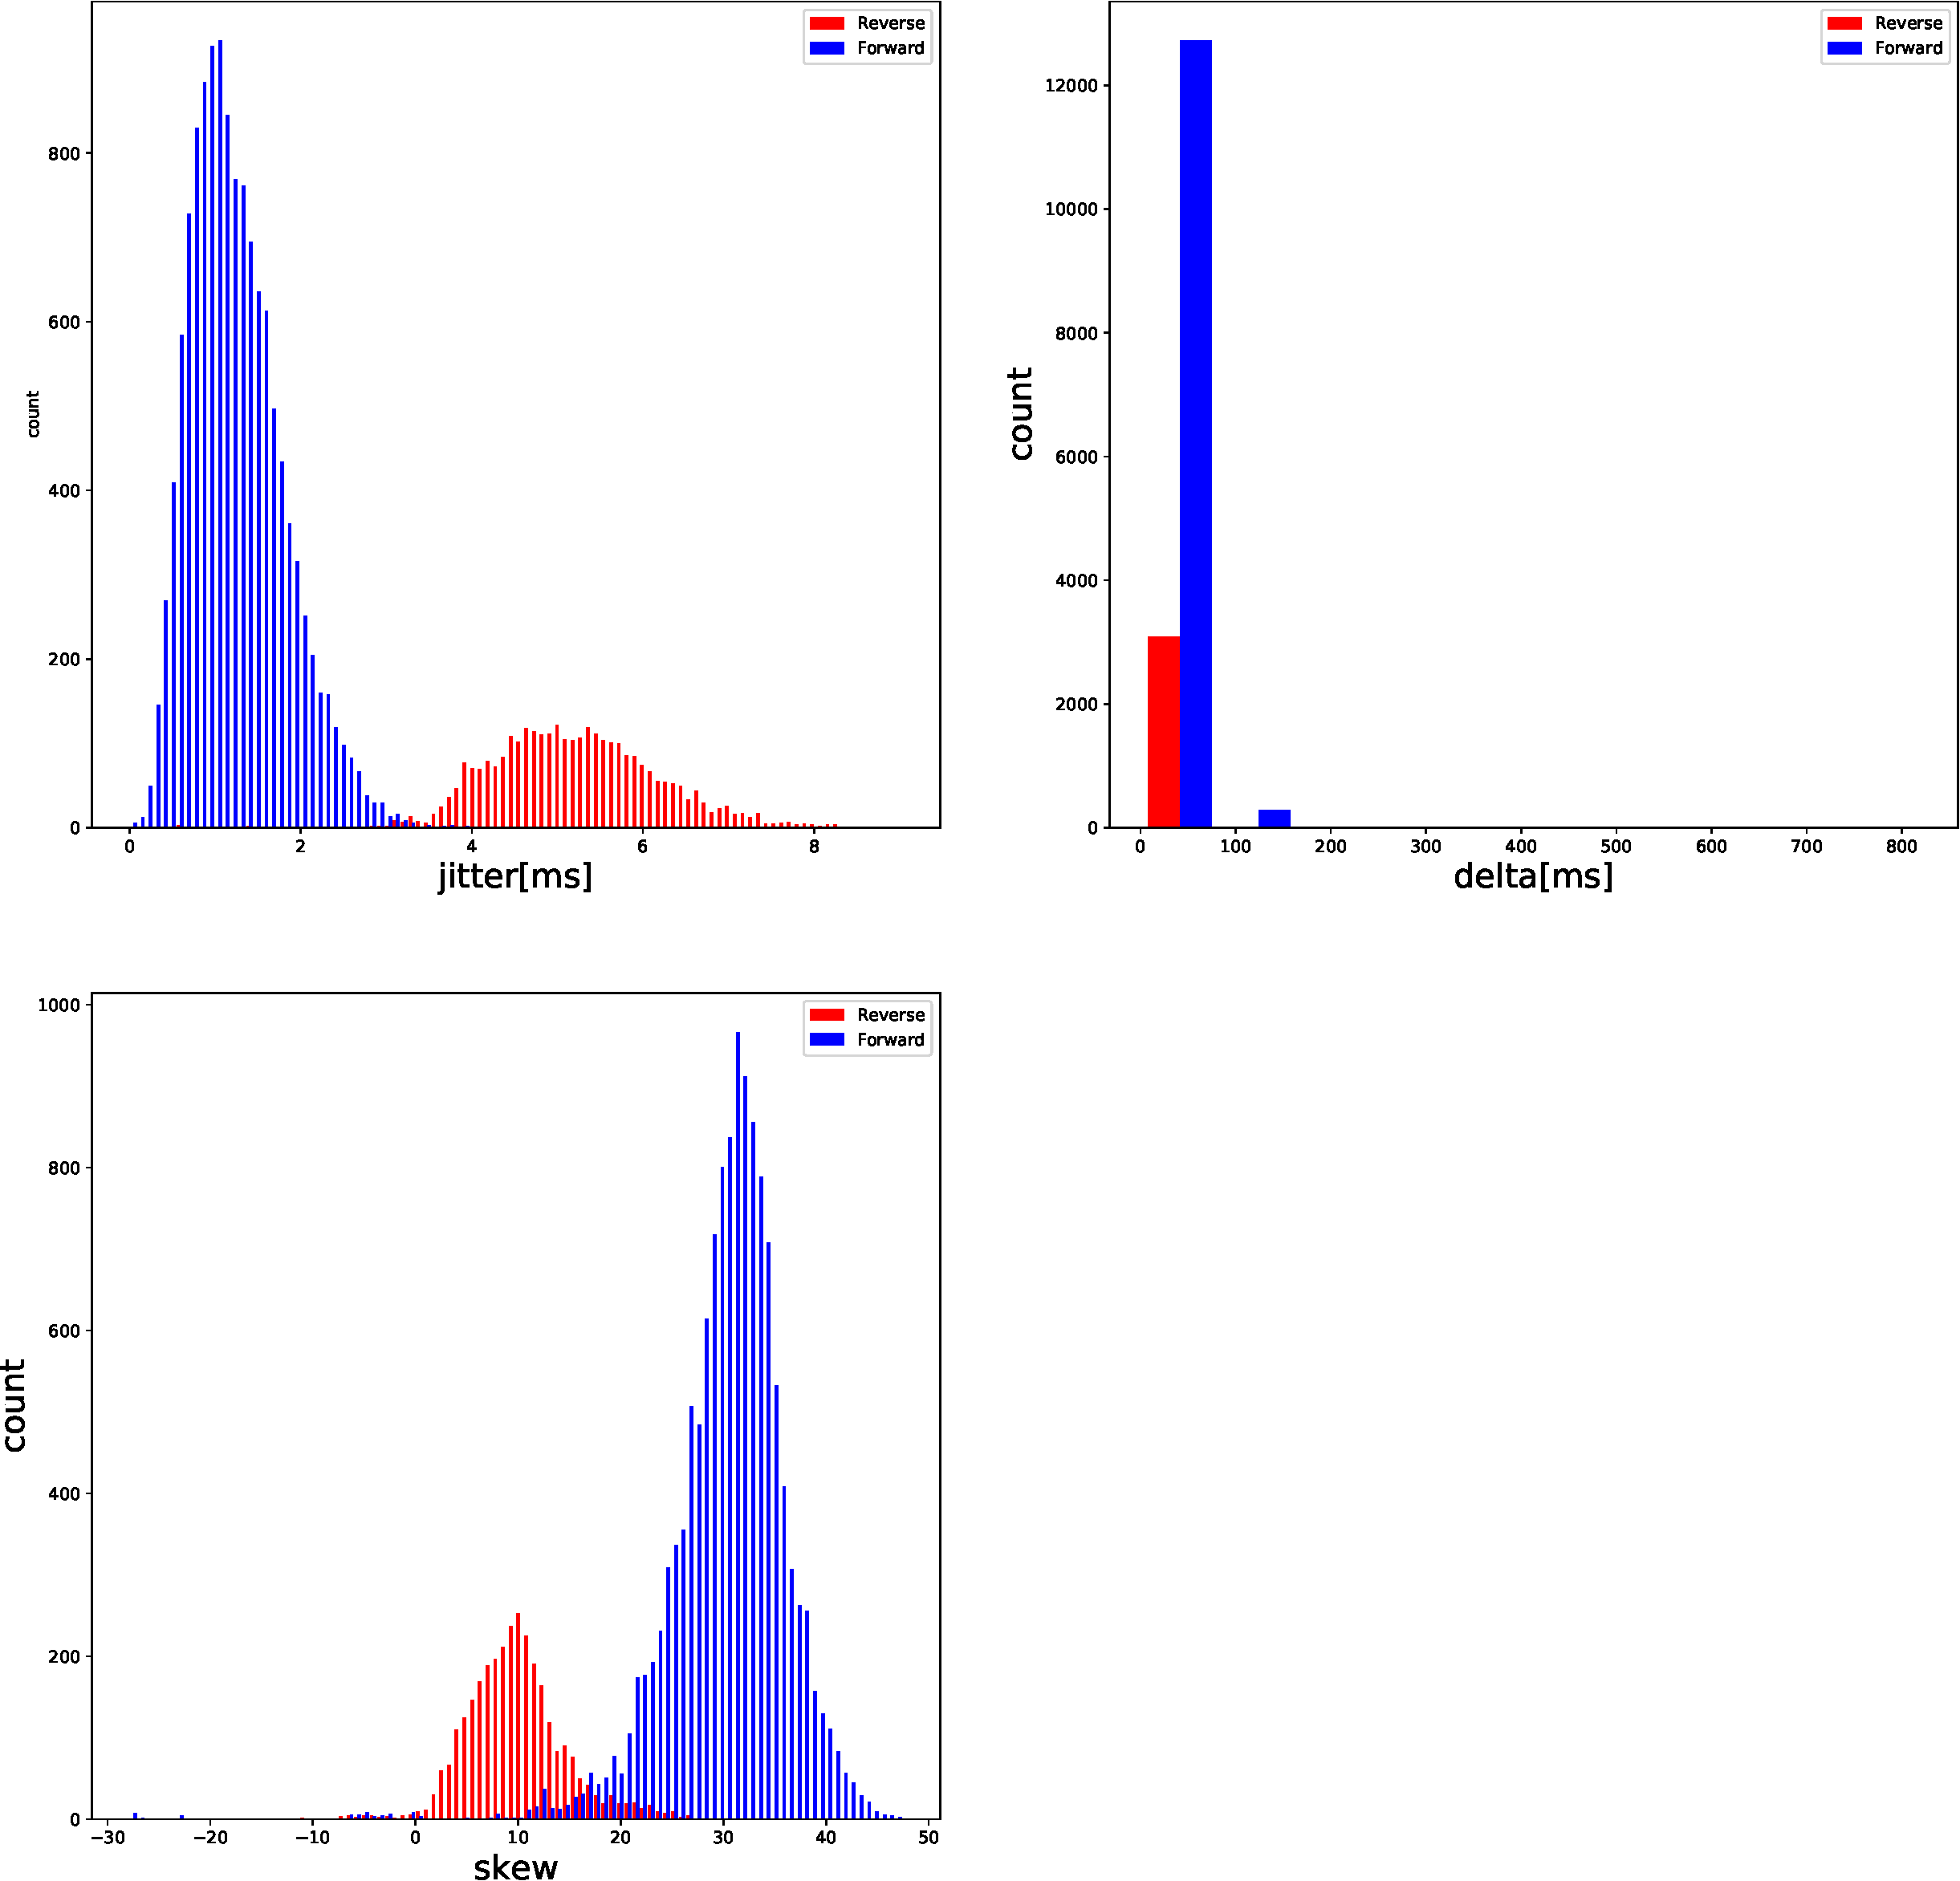
\includegraphics[width=\textwidth]{images/landline-histogram.pdf} % importing figure
	\caption{SIP signaling sequence diagram} 
	\label{fig:sigFlow} % labeling to refer it inside the text
\end{figure} 

\begin{figure}[!ht]
	\centering % centering figure 
	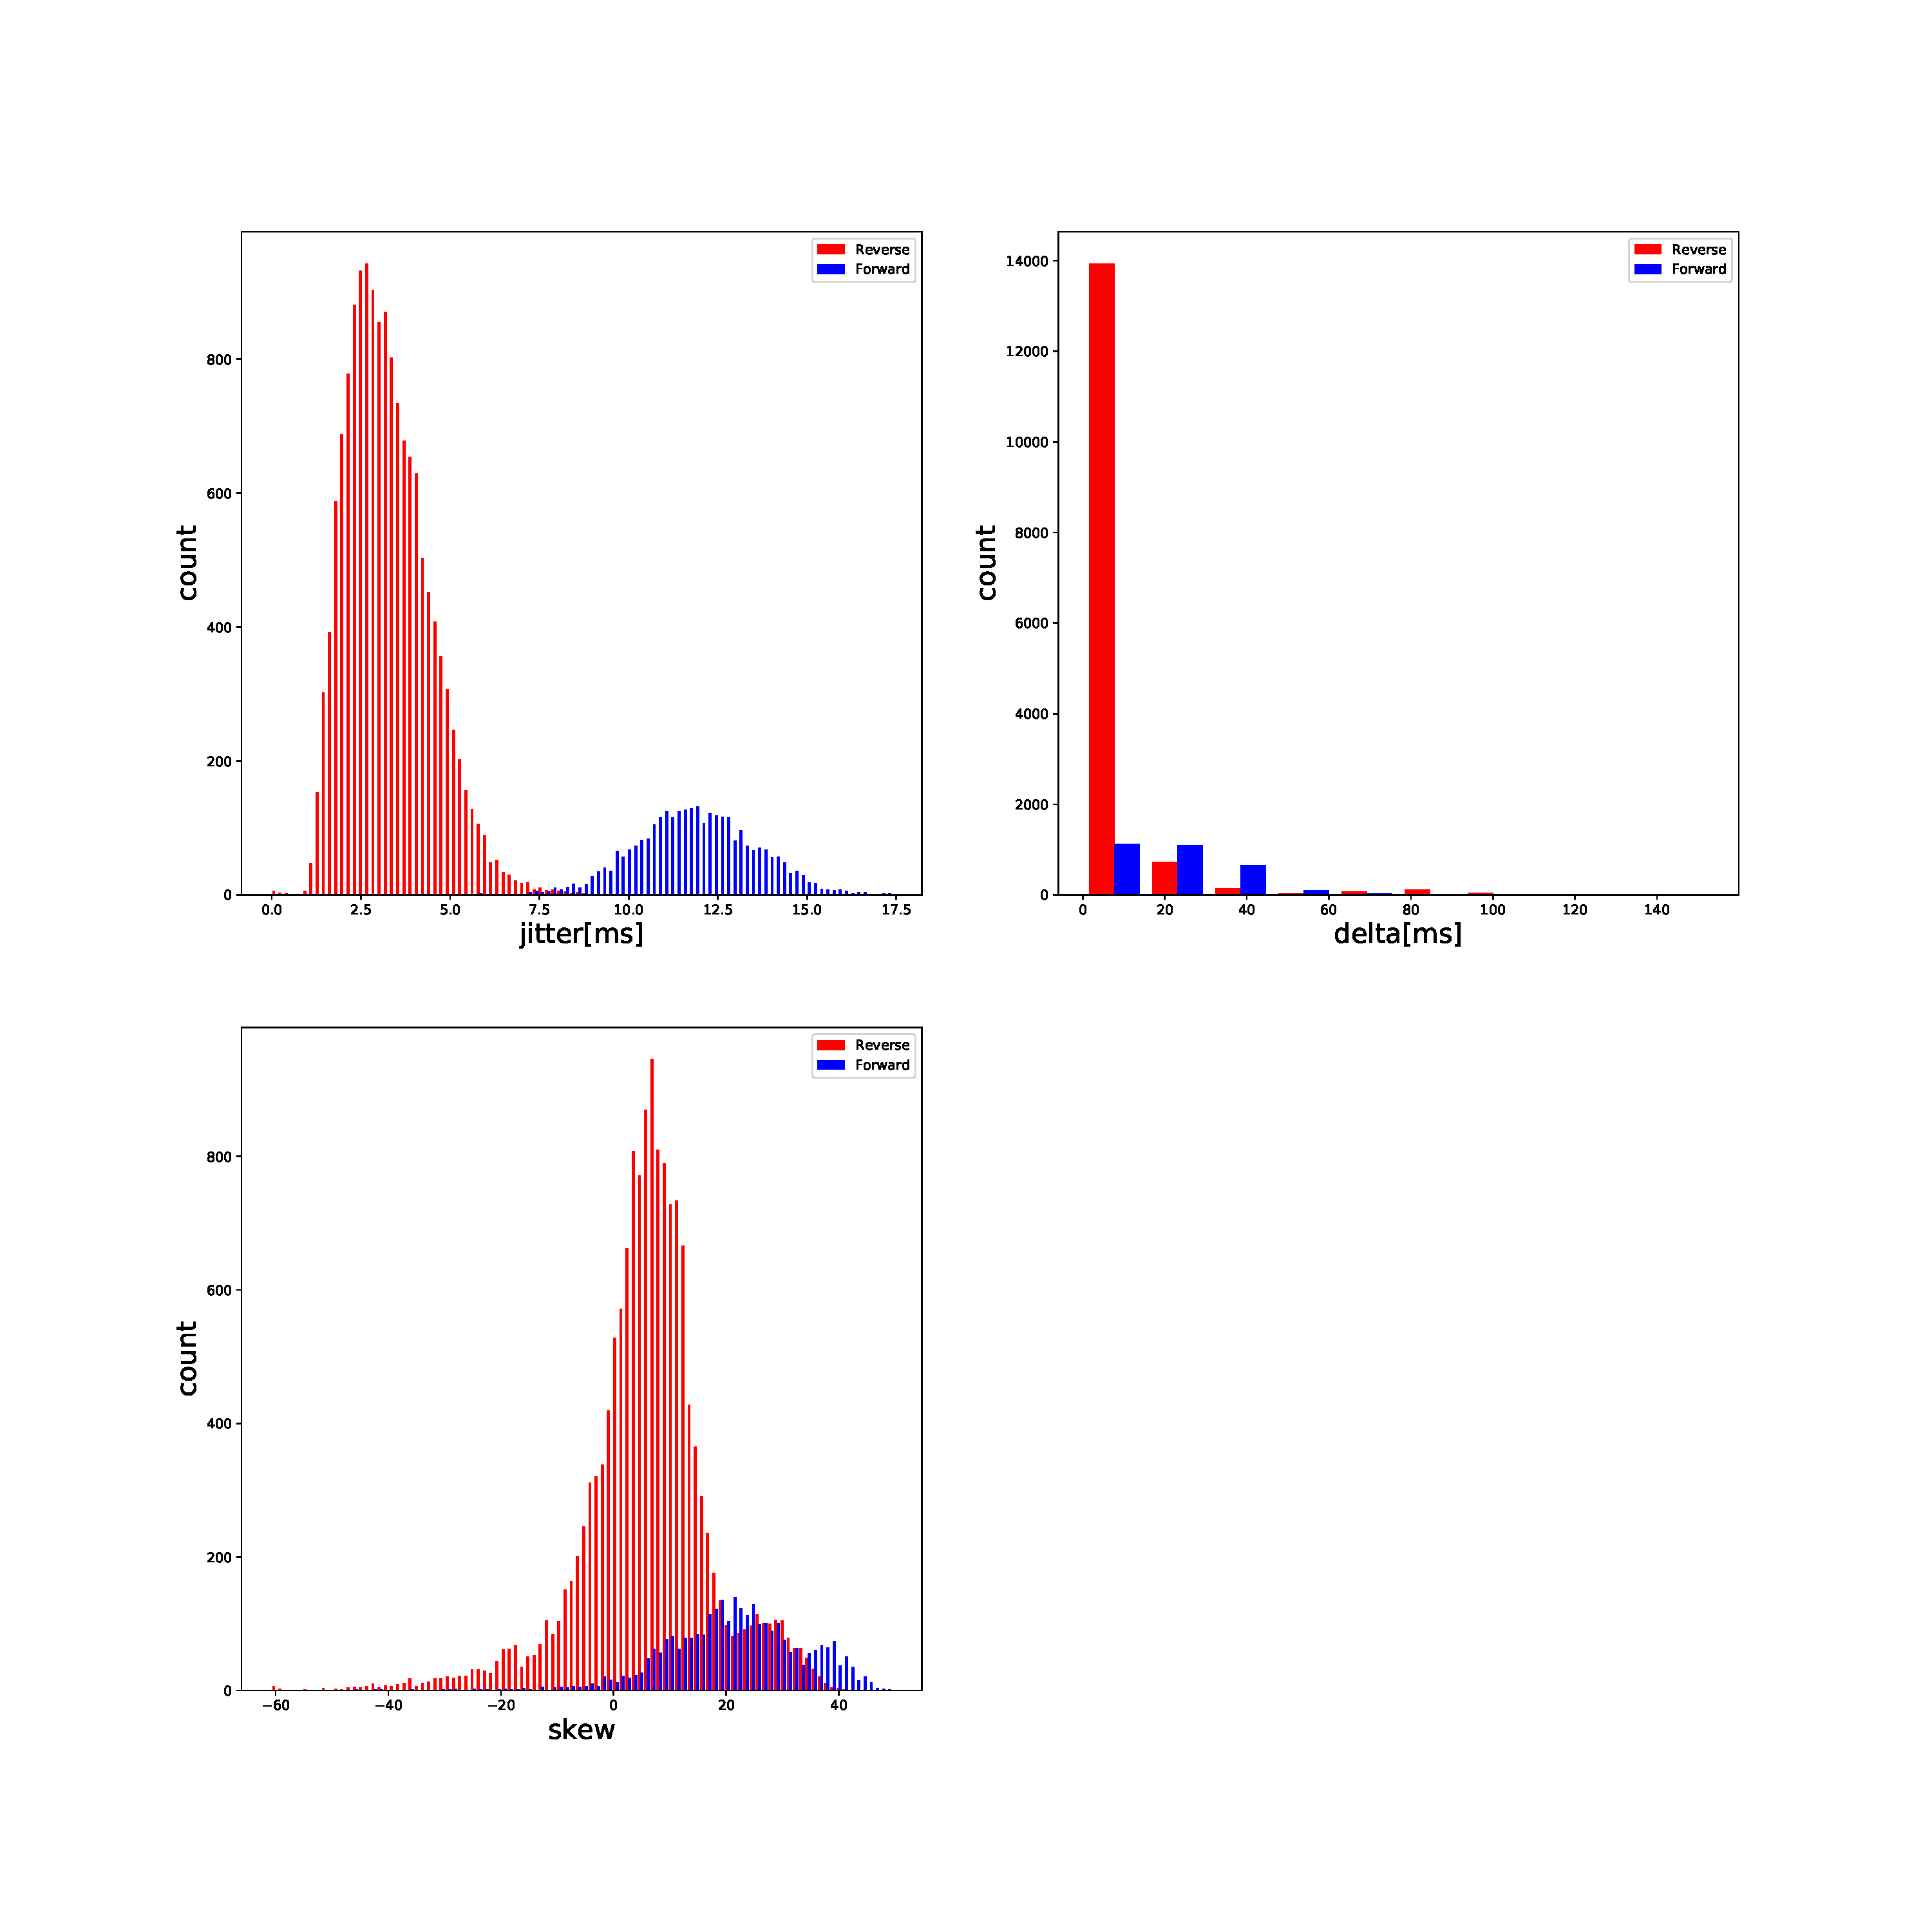
\includegraphics[width=\textwidth]{images/satelite-histogram.pdf} % importing figure
	\caption{SIP signaling sequence diagram} 
	\label{fig:sigFlow} % labeling to refer it inside the text
\end{figure} 


\subsection{Audio and video codec quality comparison} \label{subsec:audio}
For the subjective quality measurement of the audio and video experience of different codecs the rating system of the Mean Opinion Score was used.
Thereby, the quality is rated with a value between 1 (Bad) and 5 (Excellent). 
In \cref{tab:capture} all selected scores for the different codecs and connection types can be seen. 

In general, a big difference in QoS and Quality of Experience (QoE) could be observed depending on whether the connection was to the landline host or the satellite host.
This is especially noticeable when comparing the loss rate.
Connections over landline had a mean loss rate of XX and over satellite xx. 
This also explains the large differences in QoE.


%----------------------------------------------------------------------------------------
%	SECTION 3
%----------------------------------------------------------------------------------------
\section{Conclusion}

Was sind die besten Codecs für welche Situation. 
%----------------------------------------------------------------------------------------
%	SECTION X
%---------------------------------------------------------------------------------------

\printbibliography

\end{document}
